\documentclass{proc}
\usepackage[utf8]{inputenc}
\usepackage{graphicx}
\graphicspath{ {./} }
\usepackage{multicol}
\usepackage{subfig}
\usepackage{authblk}

\title{Real-time Visualization of a Distributed Peer-to-Peer Botnet}
\author[1]{Alejandro Soler Gayoso}
\author[2]{Rushdi Abualhaija}
\affil[1]{Worcester Polytechnic Institute, asolergayoso@wpi.edu}
\affil[2]{Worcester Polytechnic Institute, rmabualhaija@wpi.edu}
\date{April 30th 2019}



\begin{document}
\maketitle
\begin{abstract}
	Here is where I would say what is in this document.
\end{abstract}

\section{Introduction}
Botnets stand out as one of the largest security threats to the average user. Composed sometimes by tens of thousands of nodes, they can collectively perform massive coordinated attacks, such as Distributed Denial of Service. Traditionally, bots in the network receive their commands from Command and Control (C\&C) servers, which produced malicious commands camouflaged in regular network traffic. 


It is no easy task to bring down one of these nefarious networks, especially as the size of the botnet increases. Taking down one individual node will not serve any purpose, as there could be thousands of others still at work. However, if the C&C server were to be compromised, it could lead to the downfall of the entire botnet. However, the rise of a new type of botnet built on a distributed peer-to-peer (P2P) architecture are resilient to this approach since commands are not distributed from a single C\&C server, but rather from each node to its neighbors and so on. 


Effectively controlling these type of networks can be a rather overwhelming task. In a stealthy P2P
botnet, traffic should always take different routes, and commands should come from different origins, making the management quite a tedious and leading to inefficient routes, and partial command propagation. For that reason, we are proposing a visualization of a P2P botnet on real-time, that would optimize the its management by providing an overall view of the topology, as well as route statistics, for better propagation. 
\section{Background}

Botnets are extremely prevalent today and have already caused untold damage with their DDoS attacks and ability to silently infect and perform actions from within countless hosts. For example in 2008 the Kraken botnet was found to be present within 10\% of all fortune 500 companies and was capable of sending over 600,000 emails a day. Another aspect that makes botnets risky is the range of threats from malicious actors to bored kids such as in the case of the 2016 Mirai botnet which infected over 600,000 machines and used to DDoS attacks to make the internet inaccessible to most users on the east coast. This attack was put together by a group of kids looking to have an advantage in a videogame\cite{WhiteOps}. Even more recently botnet attack on Electrum bitcoin infected more than 150,000 user and stole \$4.6 Million in value from users wallets. Due to the prevalent and pervasive threat that botnets pose, it is important to effectively control them.

\section{Method}
P2P architectures run on top of existing networks [1]. Their decentralized fabric allows every node to act as a client and a server, and thus eliminating the need for a dedicated server and making them cheaper and easier to set up. When used as a botnet, it can be a tremendously difficult task to trace the attack back to the origin due to the distributed nature of the network. Similarly, as the size of such a network increases, it becomes harder administer it. For that reason, as well as having worked with P2P networks in the past, it seemed a good area to improve through the power of data visualization. In particular, we focus on the building a visualization capable of displaying close to real-time data about the nodes and the links of the network, as well as providing additional context-based information for every node. 

\subsection{Generating Real Data}
Since real-time data was a necessity for this project, we built and implemented a real P2P botnet with 15 bots in a controlled environment. This botnet was the responsible for generating realistic traffic that would then be utilized for the visualizations. Although the scale was not as large as typical malicious botnet, we were able to replicate the P2P distribution, avoiding any centralized C&C servers. Consequently, the two main components of this botnet are the master and the bot.

\subsubsection{Master}
As said before, there are no centralized servers that connect to all the bots, however there is a master a stateless entity which is meant to be run on the administrators host. The master keeps track of all the different bots, and it has the ability to change their status, send specific command, and even terminate the bots execution. The master is the primordial information gatherer and provider for the visualization, as it constantly shares the status of the botnet, which is used to build a visual representation. As seen in figure 1, this program looks like a normal Linux shell, offering zero contextual visualization of the botnet, making it harder to manage as size increases. 
\begin{figure}
  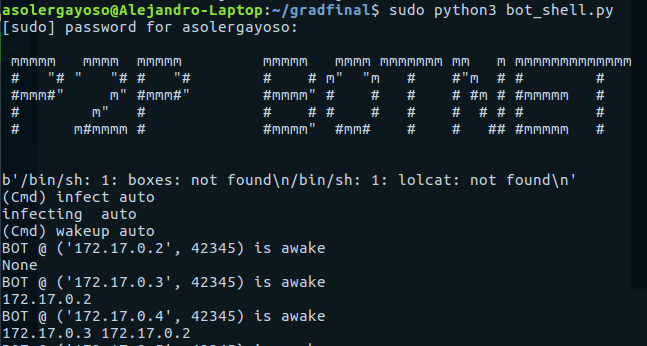
\includegraphics[width=\linewidth]{init_screen.png}
  \caption{Welcome screen of the botnet terminal.}
  \label{fig1 :node select}
\end{figure}


\subsubsection{Bot}
On the other side, each infected host is running an instance of the bot. None of the infectious capabilities were implemented as it was not in the scope of the project, and it can be dangerous. We chose to utilize docker containers in detached mode to pose as infected machines, because this virtual machines do need as much resources, allowing for more bots to run simultaneously. The containers are initialized running the bot and are all located in the same internal subnet. Each bot can have three different states: 
\begin{itemize}
    \item Ready: The bot is active and can receive, forward and execute commands. It will switch to "Asleep" upon reception of a sleep signal.
    \item Asleep: This is a more stealthy mode, where the bot will remain silent unless it receives a wake up signal from the master, in which case it will switch to the "Ready" state. 
    \item Unreachable: The bot has been disconnected from the network.
\end{itemize}
At first, the bot is initialized with the "Asleep" state, until the master sends a "wakup" signal, upon which the state is changed to "Ready". Once the bot is in "Ready", the master will be able to start sending commands. If a master wants to propagate a command throughout the entire network, it will only need to send the an "execute" message to any of the bots. When a "Ready" bot receives an execution command from the master, it will execute it in the host first, and then it will forward the command to its neighboring bots, which will repeat the process with their neighbors. This is possible when the bot is awaken, it also receives a list with a few of the "Ready" that it wil connect to, as neighbors. The beauty of the P2P architecture makes it possible to spread a message through an entire network, from a single node, and it could be a different node every time. That is why it can be so hard to track the master behind the P2P botnet.  


\subsection{Inter-Process Communication}
As a real-time visualization, one of the greatest challenges was to provide a representation of the state of the network as fast as possible. We decide to have the visualization read from a CSV file, that gets continuously updated by the botnet. Logically, having 15 bots, one master read and write to a file can add considerable overhead to the overall execution, not mentioning potential mutual exclusion issues that occur when multiple process try to read and write to the same file. 

To solve this issue, we first reduced as much as possible the number of times the bots write to the file, so that the master is the primary editor of that file. Moreover, it took careful scheduling of all the writes and read, and well as the "lockfile" python module to solve any concurrency issues between all the different threads. Additionally, in order to improve the efficiency in the status queering between the master and the bots, we added additional threads running constantly in the background connected through a different port..
\begin{figure}
  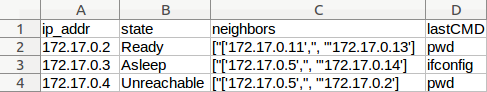
\includegraphics[width=\linewidth]{CSV.png}
  \caption{File with the state of the botnet.}
  \label{fig1 :bots.csv}
\end{figure}

\subsection{Visual Representations}
Similarly to [4] all the possibilities we considered to visualize the topology of the network were in the realm of node-link and adjacency diagrams. In particular, one the of the questions that we asked at the beginning was whether a P2P botnet carries some sort of intrinsic hierarchy that could be represented through hierarchical force layouts. Among the potential advantages of using hierarchies, we find the ability to mimic real path selection algorithms[4]. Nonetheless, P2P networks and especially botnets are highly dynamic networks [1] that are constantly adapting to new changes in the environment to ensure some level of robustness. Hence, hindering the natural formation of hierarchical structures, and therefore establishing the master-slave relation as the sole difference. Consequently, when visualizing the nodes, we avoided depicting any hierarchy, by representing all the nodes with the same shape and size.  

\begin{figure}[!tbp]
  \centering
  \subfloat[Nodes have been initialized but remain unreachable.]{\resizebox{.3\textwidth}{!}{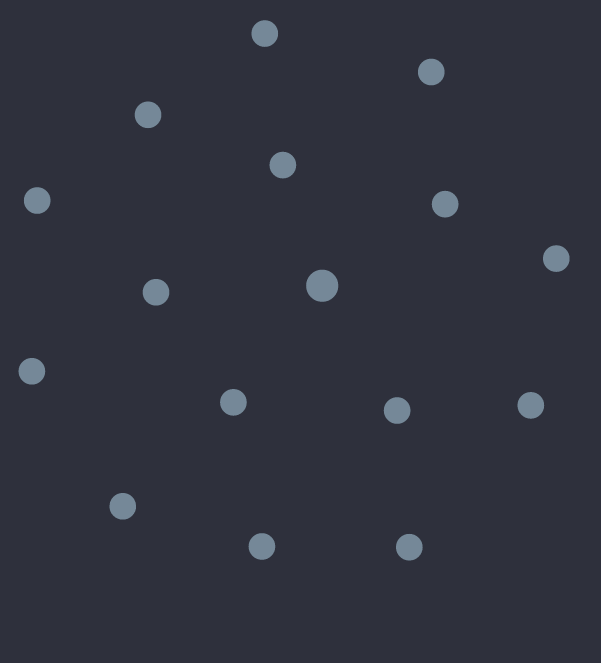
\includegraphics[ width=0.5\textwidth, scale = 0.5]{topo_init.png}\label{fig:f1}}}
  \hfill
   \subfloat[Nodes are infected by master in the 'Asleep' state.]{\resizebox{.3\textwidth}{!}{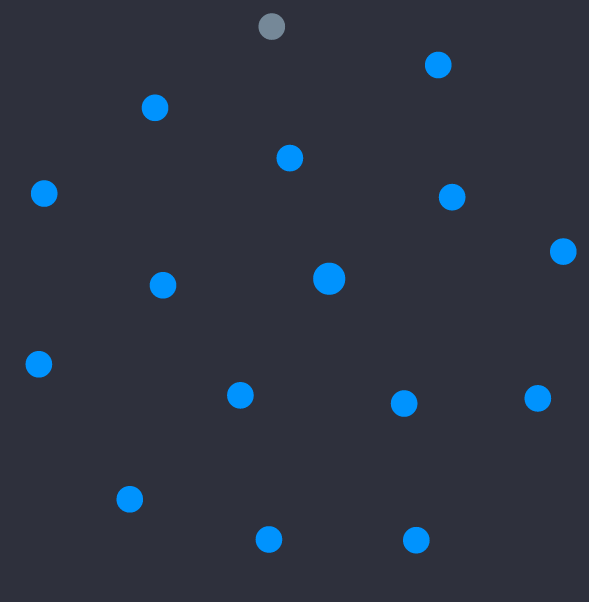
\includegraphics[width=0.5\textwidth]{topo_asleep.png}\label{fig:f1}}}
  \hfill
  \subfloat[Some of the nodes have been awaken.]{\resizebox{.3\textwidth}{!}{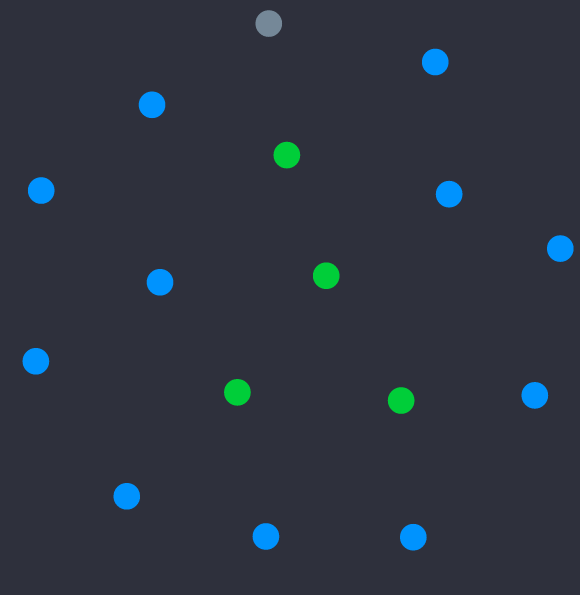
\includegraphics[width=0.5\textwidth]{topo_waking.png}\label{fig:f2}}}
  \caption{Real-time view of the botnet boot sequence.}
\end{figure}


Additionally, we pondered whether all the links between the nodes should be included in the visualization, as it poses a trade-off between structural information of all the links and gains in readability. This question ties back to the previous one, as the ever changing topology and lack of hierarchy makes the distinction between links' relevance rather ambiguous. As a result, considering the reduced size of our botnet, we decided to include all links in the visual representation. This decision however came at some cost, namely the added overhead that it takes when parsing all the neighbors of a given node. 

\subsubsection{State of the Network}
After taking into account the different considerations mentioned before, we proceeded to create a visualization that accurately represented the state of the network in real-time. As shown in Figure 6a, the master can query the state of the network at any point in time, however, the text output is quite unpractical to quickly understand the topology and the state of the nodes. For that reason, we a dynamic network graph using a force layout, that draws all the nodes as circles on the screen and connects them to each other, based on each of their "neighbors" fields. Additionally, each node is color filled with a different color depending on its state, blue being "Asleep", green "Ready, and grey "Unreachable". Figure 3 how the boot sequence of the botnet can be visualized in real-time. At first, all nodes are initialized but unreachable, depicted as disconnected grey circles, see Figure 3a. In the next step of the seqeuence, the nodes have been recognized by the master with the "infect" signal and given the 'Asleep' state, therefore their color changes to blue, see Figure 3b. At the instant captured in Figure 3c, some nodes had been awoken by master, but the links had not be drawn in the screen. Finally, Figure 4 shows a representation of the botnet at a given time after initialization, when one of the nodes was "Asleep" (blue), another node was "Unreachable" (grey and disconnected from the botnet), and the rest are "Ready"(green). Any changes applied on the botnet will be immediately be reflected on the visualization.

\begin{figure}
  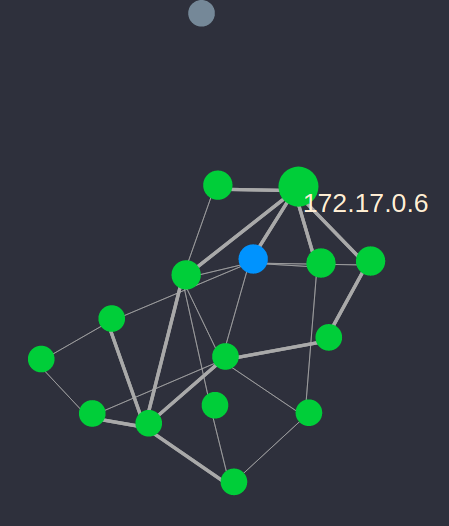
\includegraphics[width=\linewidth]{network_graph.png}
  \caption{File with the state of the botnet.}
  \label{fig1 :bots.csv}
\end{figure}

Previously, we concluded that discriminating between links based on relevance was quite ambiguous, especially due to the dynamic nature of the network. However, it is possible to visualize links differently based on the amount of traffic each link carries. In Figure 3b certain links are thicker than other, as they have recently passed the most recent command. Of course, at this scale and with this amount  of traffic this link representation changes all the time and is not very practical, but on a larger scale, it could help the administrator identify certain common routes between the nodes.

\subsubsection{Node-specific Context}
The user can also directly interact with the visualization by using the mouse pointer. As seen in Figure 3b, by placing the cursor on a node, the ip address of that node will be displayed, followed by an increase in the size of the node, as well as all its direct links. Moreover, by clicking on the specific node, the context will focus to the selected node by changing its color, as well as the color of its links and directly connected nodes to black, see Figure 4. 

Although implementation for this part was not completed, including coordinated multiple views with an additional visualization would enhance the contextual information given to a selected node. In particular, we had thought of displaying a table with all the previously executed commands, as
well as line chart with the throughput of the node against time.

\begin{figure}
  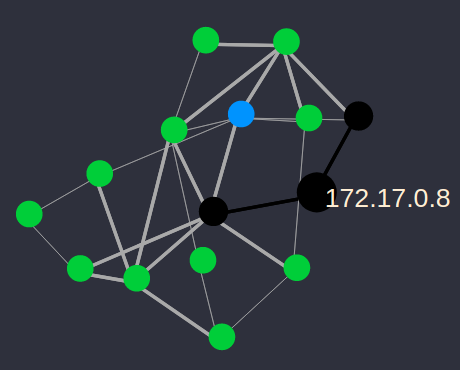
\includegraphics[width=\linewidth]{network_select.png}
  \caption{Selecting a node displays all the direct path of the node.}
  \label{fig3 :node select}
\end{figure}


\section{Evaluation}
This section, we will evaluate our visualization using use cases and performance measures. This evaluation procedure was inspired by [1].

\subsection{Performance measures}



Both the botnet and the visualization was run simultaneously on a signle laptop, running 64-bit Ubuntu 16.04 LTS with an Intel Core i7-4700MQ CPU adn 8GB of RAM. Since the different components of the botnet and the visualization would not be run on the same host in a real setting, we discarded running CPU performance statistic. On the other hand, we focused on network statics in particular the amount of incoming bytes on the hosts docker interface, in other words, the bytes received by the master. We believe that this metrics provided more useful data to identify potential bottlenecks, and recognize patterns in network flow.

\begin{figure}
\centering
  \resizebox{.5\textwidth}{!}{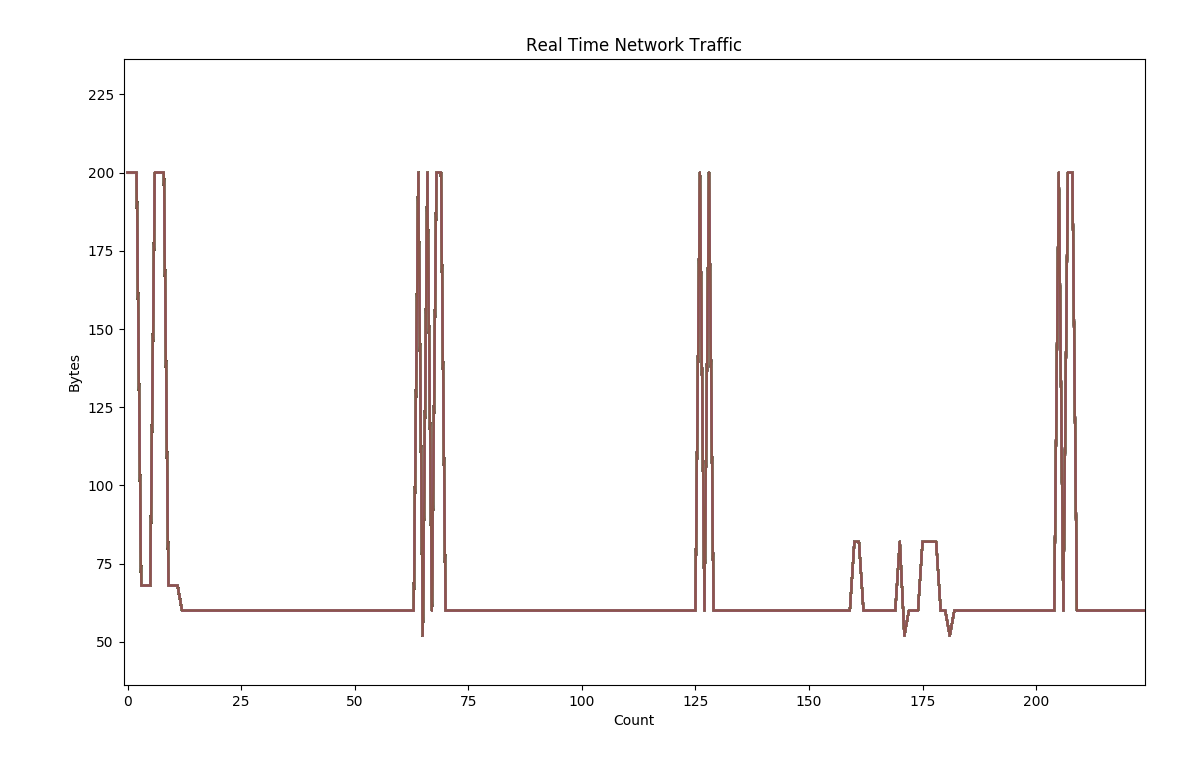
\includegraphics[width=\linewidth]{network_metrics.png}}
  \caption{Traffic Flow of the botnet.}
  \label{fig1 :bots.csv}
\end{figure}

Figure 7 shows the byte flow received by the docker network interface over a period of time. There are four different peaks that reach the 200 bytes which correspond to a new node awakening and joining the rest of the botnet. Moreover, between the third and fourth peaks, we see a small fluctuations that barely reach 80 bytes. These corresponds to commands being sent by the master to a node. Finally, there seems to be a base load at 60 bytes. This corresponds to the continuous background update between the master and the nodes, vital to the accuracy and responsiveness of the visualization. 


\subsection{Use cases}
The underlying purpose of this project was to create an accurate and responsive visualization of a distribute P2P network that would greately simplyfy the cumbersome task of managing it. As seen in Figure 7a, the botnet terminal provided the state of the nodes and the topology of the botnet in a text format. Even with 15 nodes, which a relatively small botnet, it was already hard to get a clear picture of the topology from the terminal. Scale up to a 1000-node network and the topology in text format becomes useless. 

From our experience, this tool makes the process of reacting to changes and having a clear and update topology much easier. In Figure 7, we contrast the difference in reading topology. There is clear added value in using tool on top of an existing P2P network. Additionally, it is proven to be valuable for non-experts in P2P network, as it provides a fairly intuitive picture of the state of the network. 

\begin{figure}[!tbp]
  \centering
  \subfloat[State of the network seen on terminal.]{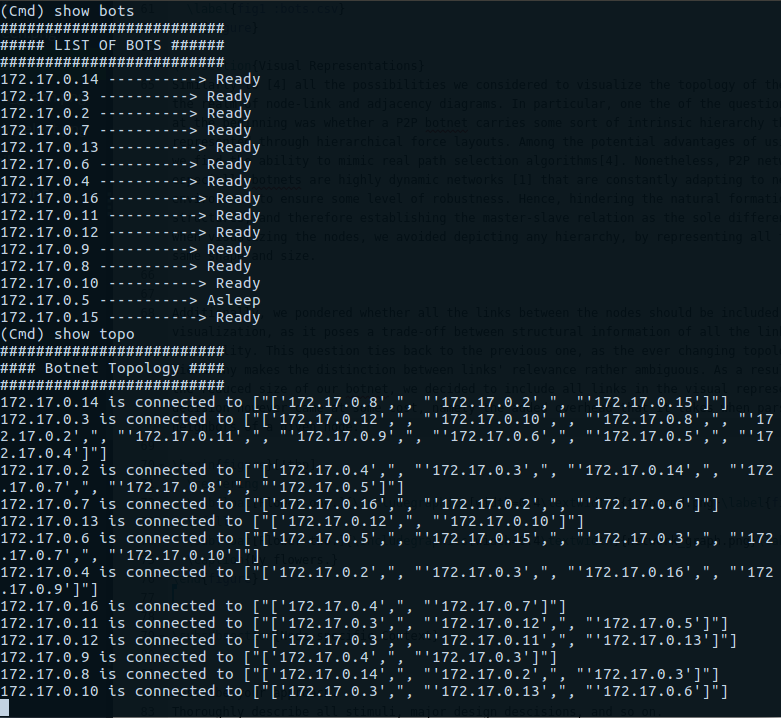
\includegraphics[width=0.4\textwidth]{topo_cmd.png}\label{fig:f1}}
  \hfill
  \subfloat[State of the network seen on Visualization.]{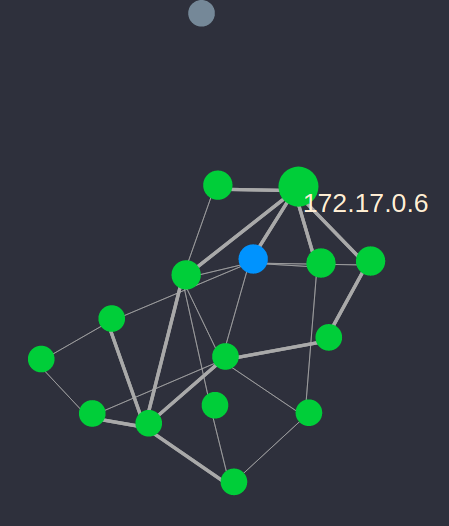
\includegraphics[width=0.4\textwidth]{network_graph.png}\label{fig:f2}}
  \caption{Dramatic improvement of real-time state of the network understanding.}
\end{figure}

\section{Discussion}


\section{Conclusion}


\nocite{*}

\bibliographystyle{abbrv}
\bibliography{paper}

\end{document}
